%!TEX TS-program = xelatex
\documentclass[12pt,a4paper]{report}
\usepackage[utf8]{inputenc}
\usepackage{upquote}
\usepackage{dirtree}
\usepackage{listings}
\usepackage{color}
\usepackage{fancyhdr}
\usepackage{titlesec, blindtext, color}
\usepackage{amsmath}
\usepackage{graphicx}
\usepackage{physics}
\usepackage{csvsimple}
\usepackage[hyphens]{url}
\usepackage{hyperref}
\usepackage{booktabs}
\usepackage{tabularx}
\usepackage[margin=0.8in]{geometry}
\usepackage{float}
\usepackage{subfig}
\usepackage{listings}
\usepackage{upgreek}
\usepackage[american]{circuitikz}
\usepackage[titletoc,title]{appendix}
\usepackage{amssymb}
\usepackage{array,etoolbox}
\usepackage[parfill]{parskip}
\usepackage{ragged2e}
\usepackage{pgfplots}
\usepackage{pdfpages}
\usepackage{svg}
\usepackage{lastpage}
\usepackage{todonotes}
\usepackage{xcolor}
\hypersetup{
    colorlinks,
    linkcolor={red!50!black},
    citecolor={blue!50!black},
    urlcolor={blue!80!black}
}
\pgfplotsset{width=10cm,compat=1.9} 
\usepgfplotslibrary{external}
\tikzexternalize 

\newcommand{\hsp}{\hspace{20pt}}
\titleformat{\chapter}[hang]{\Huge\bfseries}{\thechapter\hsp}{0pt}{\Huge\bfseries}

\preto\tabular{\setcounter{magicrownumbers}{0}}
\newcounter{magicrownumbers}
\newcommand\rownumber{\stepcounter{magicrownumbers}\arabic{magicrownumbers}}
\newcommand{\ruler}{\noindent\rule{\textwidth}{1pt}}

% Standard colors for the code syntax highlighting.
\definecolor{pblue}{rgb}{0.13,0.13,1}
\definecolor{pgreen}{rgb}{0,0.5,0}
\definecolor{pred}{rgb}{0.9,0,0}
\definecolor{pgrey}{rgb}{0.46,0.45,0.48}

\def\doubleunderline#1{\underline{\underline{#1}}}
\newcommand{\doubleindent}{\indent \indent}

% Define Y colymntype
\newcolumntype{Y}{>{\centering\arraybackslash}X}

\definecolor{mygreen}{rgb}{0,0.6,0}
\definecolor{mygray}{rgb}{0.5,0.5,0.5}
\definecolor{mymauve}{rgb}{0.58,0,0.82}

\lstset{ 
  backgroundcolor=\color{white},   % choose the background color; you must add \usepackage{color} or \usepackage{xcolor}; should come as last argument
  basicstyle=\footnotesize,        % the size of the fonts that are used for the code
  breakatwhitespace=false,         % sets if automatic breaks should only happen at whitespace
  breaklines=true,                 % sets automatic line breaking
  captionpos=b,                    % sets the caption-position to bottom
  commentstyle=\color{mygreen},    % comment style
  deletekeywords={...},            % if you want to delete keywords from the given language
  escapeinside={\%*}{*)},          % if you want to add LaTeX within your code
  extendedchars=true,              % lets you use non-ASCII characters; for 8-bits encodings only, does not work with UTF-8
  frame=single,	                   % adds a frame around the code
  keepspaces=true,                 % keeps spaces in text, useful for keeping indentation of code (possibly needs columns=flexible)
  keywordstyle=\color{blue},       % keyword style
  language=C,                      % the language of the code
  numbers=left,                    % where to put the line-numbers; possible values are (none, left, right)
  numbersep=5pt,                   % how far the line-numbers are from the code
  numberstyle=\tiny\color{mygray}, % the style that is used for the line-numbers
  rulecolor=\color{black},         % if not set, the frame-color may be changed on line-breaks within not-black text (e.g. comments (green here))
  showspaces=false,                % show spaces everywhere adding particular underscores; it overrides 'showstringspaces'
  showstringspaces=false,          % underline spaces within strings only
  showtabs=false,                  % show tabs within strings adding particular underscores
  stepnumber=1,                    % the step between two line-numbers. If it's 1, each line will be numbered
  stringstyle=\color{mymauve},     % string literal style
  tabsize=4,	                   % sets default tabsize to 2 spaces
  title=\lstname                   % show the filename of files included with \lstinputlisting; also try caption instead of title
}

% Group name
\newcommand{\groupname}{Group}

% Define author information
\newcommand{\authors}{Philip Hjortsberg, William Wennerström}
\newcommand{\authorsinfo}{
    Hjortsberg, Philip\\
    \texttt{\href{
        mailto:phihjo-2@student.ltu.se
    }{\color{black}{
        phihjo-2@student.ltu.se
    }}}
    
    \and
    
    Wennerström, William\\
    \texttt{\href{
        mailto:wenwil-5@student.ltu.se
    }{\color{black}{
        wenwil-5@student.ltu.se
    }}}
}

% Define course information
\newcommand{\coursename}{Design of Dynamic Web Systems}
\newcommand{\coursecode}{M7011E}

% Define project name
\newcommand{\projectname}{Project Roaster}

% Define information about the school/university
\newcommand{\schoolinfo}{Department of Computer Science, \\
                         Electrical and Space Engineering \\
                         \bigskip{}
                         Luleå University of Technology \\
                         Luleå, Sweden
}

\title{
    \coursecode{} \\
    \coursename{} \\
    \vspace{1.8em}
    % ~~Tinder~~ Roaster logotype
    \begin{figure}[H]
      \centering
      \includesvg[width=2cm]{logotype.svg}
    \end{figure}
    \textbf{\projectname{}} \break
    \author{
        \authorsinfo{}
    } \break{}
    \schoolinfo{}
    \vspace{1.8em}
    \begin{figure}[H]
      \centering
      
\includegraphics[width=5cm]{LTU.jpg}
    \end{figure}
}

\renewcommand\footnotemark{}
    \date{\today}
 
\pagestyle{fancyplain}
\renewcommand{\headrulewidth}{0pt}
\renewcommand{\footrulewidth}{0pt}
\lhead{}
 
\begin{document}

\maketitle
\thispagestyle{empty} % Disable page numbers for this page.
\newpage

{\hypersetup{linkcolor=black}
    \tableofcontents}
\newpage

%\listoftodos
%\todo[inline]{Remove \texttt{\textbackslash{}listoftodos} before hand-in}
\newpage

\chapter{The problem}
One of the big pains when programming in groups is code that is unreadable. Many times you can look at a code snippet and see who wrote that piece
just based on the formatting and comments. The solution to this is to enforce an uniform code and documentation style that every person adheres to.
This is normally done by installing a linting tool chain and configuring it equally on all systems used for developing.
The idea for this project is to eliminate the installing and configuring step by doing it all with the site called Roaster Inc. (\url{https://roast.software}), along with the intriguing feature of following your own and friends code quality progress.

Roaster analyzes and grades your code. The user can register and follow their personal programming progress and compare it with people they follow - you could compare it to music scrobbling, but for code! Personal statistics is generated by running static code analysis on the uploaded code - data such as number of errors, number of warnings and even code style problems is collected. The statistics can then be viewed in a feed where both your own and the people you follows progress is listed. Global statistics like number of errors and warnings and number of rows analyzed is displayed on a page that can be viewed by everyone.

% \todo[inline]{Jag tror inte jag riktigt förstår vad denna paragrafen försöker säga, är det...
% As the website is thought to be forth most educational, no formatting is done on the code and is left as an exercise for % the user.
%
%}
% The site is thought to be forth most educational, in this scenario it means that the solution is perfectly capable of doing the formatting and linting for the student / user, but then they would not learn what kind of style errors 
% or semantic improvements was made. Therefore does the online web application only list the errors and warnings, with precise origin in the source code as an exercise for the student / user to fix.

A typical user scenario could be that a teacher is sick and tired of reading spaghetti code made by novice students and would rather let them learn that readability and an uniform code style is important. But that takes time to teach, and the teacher has to focus on the actual subject of the course.

Instead, the teacher can tell the students that they have to Roast\textsuperscript{\textregistered} their code and get no warnings and errors before submitting the work!

The students increases their code quality and the teachers are happier!

\chapter{Technology choices}
The participants of the course were encouraged to learn new technologies and tools that the developers had never used before or wanted to learn more about. The technologies chosen all was chosen with scalability and security in mind, whenever applicable the developers chose enterprise grade software.

\section{Database}
In order to choose the right database for a project the designers need to consider what type of data that is to be stored and if availability (NoSQL) or robustness (SQL) is of utmost importance.
Considering the aspects above the developers chose robustness, a SQL database should be the best choice for this type of application where mainly structured data is stored. 

While designing the system, the developers wanted the database to handle objects with strict value types (domains), hence a Object Relational Database (ORD) was desired and PostgreSQL has good support for advanced features for object handling and custom definition of objects. PostgreSQL is also fully ACID compliant\cite{pg-acid} which is desired. PostgreSQL has the ability to use advanced data constraints which enables better robustness. PostgreSQL also has good conformance with the SQL standard\cite{pg-sql-conformance}. PostgreSQL is one of the most advanced and fastest databases\cite{db-benchmark} that is free to use and open source.
One of the two developers in this project had prior experience with PostgreSQL but only shallow knowledge which also made it interesting as a technology to learn more about.

One of the advanced features PostgreSQL has is its \texttt{HSTORE}, the ability to store sets of key/value pairs within a single PostgreSQL value\cite{pg-hstore}, comparable to an hash table. During the design phase the developers thought this feature would be good to have when storing the messages\footnote{Warnings and errors for Roast submissions.} but as it turns out, it was not necessary, as explained in \autoref{sec:database-messages}.

Competing technologies that we discarded due to the following drawbacks.
\begin{itemize}
    \item MySQL ignores \texttt{CHECK} constraints\cite{mysql-check-constraint}, requires writing advanced triggers to emulate \texttt{CHECK} instead\cite{mysql-emulate-check}.
    \item SQLite is primarily for embedded systems or low to medium volume websites and doesn't scale\cite{sqlite-when-to-use}.
    \item MariaDB doesn't offer the same amount of data integrity out of the box as \\ PostgreSQL\cite{mariadb-data-integrity}, up to the user to implement it correctly. 
\end{itemize}

\section{Session store}
A shared session store allows the web server to scale up and down with instances and still have access to the same session store as the other instances.

To save and retrieve sessions in a speedy fashion a fast in memory key/value database is used. The choice is Redis, an advanced software made for horizontal scaling by clustering. It's superior to Memcached in key names, whereas Memcached only supports 250 bytes of plain strings\cite{memcache-key-size}, Redis handles key/values to be as big as 512 MB\cite{redis-key-size} and any kind of binary data. Redis is also more modern and up to date which makes it more popular and a more relevant technology to learn\cite{key-value-comparison}\cite{redis-vs-memcached}.

\section{Containerized web server}
Docker\cite{why-docker} is not required to run the web server, it is able to run in both Linux and Windows host environments. AWS also support running the web server on ``bare metal", but was deemed to hard and time consuming to setup as the developers had no experience with this since before. Instead Docker is used to create a minimal environment that is capable of running the web server on AWS.

The Docker containers are also run in the CI/CD\footnote{Continuous Integration, Continuous Deployment} Travis CI pipeline before the actual deployment to AWS to ensure that the images work correctly. Docker offered a great experience when it comes to the deployment. Due to the testing of the images before deployment no compile errors was encountered when deploying to the live environment.

Docker also offered a great experience during the development on the developers local machines. Development took place on both a Windows and a Gentoo Linux machine so to make the setup of the databases easier they were run using Docker containers.

\section{Go web server}
To acquire more in depth knowledge of a web servers inner workings we chose to write the server without a framework. The language of choice is the Go language (hereby referred to as only Go) since it has a solid foundation as a web server language and that one of the developers had some prior experience with writing a HTTP web server with just the standard \texttt{net/http} package. To facilitate somewhat faster development and to not have to do everything from scratch the developers chose to use an existing URL router built in Go, called \texttt{gorilla/mux}.
The Go language also has good support for connecting to SQL databases through their standard \texttt{database/sql} library, such as PostgreSQL using the \texttt{pq} driver\cite{go-pq-driver}.

\newpage
\section{Hosting platform}
To have a good uptime and availability the solution needs to be deployed on a platform that supports these constraints. The developers had the following possibilities:

\begin{itemize}
    \item To host on personal hardware in a student maintained data center called LUDD. This would ensure that enough resources are available for the application since the hardware is decent. Potential downside was the up time, the facility has recently had problems with stability which is a major factor. These statements are purely subjective and based on previous experiences the developers had with servers being shut down without warning due to overloaded electrical infrastructure at the hosting location.
    \item To host on Virtual Machine provided by LUDD, as previously stated the stability is a major factor and therefore not used.
    \item Cloud infrastructure, due to the fact that the authors are students, they had access to various cloud solutions for free and due to that cloud based experience is valued in the market today, the choice was made to implement the solution in the cloud.
\end{itemize}

Choosing the cloud platform is not easy, determining if you want PaaS, IaaS or some hybrid took a while. In the end it came down to maturity, scalability and where the developers had enough credits to run the solution. Amazon Web Services (AWS) offered a solution called Elastic Beanstalk (EB)\cite{what-is-eb} which is a hybrid PaaS with automatic scaling which is used as the platform for the application. The web server that runs in a Docker container resides in an AWS EC2 instance that is managed by EB. The databases are hosted in a Amazon Relational Database Service (RDS) which is a SaaS in AWS.

Amazon Elastic Beanstalk also incorporates Amazon Elastic Load Balancing, a managed load balancer, which is what makes scaling really simple when using multiple web servers.

Due to the technology choices being deliberately chosen to be platform independent, a change of cloud provider or move to physical hardware should be a relatively simple task.

\section{Frontend language}
The course aims at using state of the art technologies, the developers wanted to explore this in as many aspects as deemed possible. The frontend language had the requirements of being fast, short learning curve, modern and something that they had not yet used. Other aspects that were highly desired were better type safety.

Strictly typed languages like Elm is functional but was discarded due to the learning curve of such a language did not suite the time budget for the project.
JavaScript was the second choice since it has many new interesting features since the ES6 release. This would however not fulfill the desire to use a type strict language.
TypeScript\cite{typescript} is a super set of JavaScript and compiles to plain JavaScript, meaning that TypeScript itself is not something that can run in a browser before its compiled. One could use the abstraction of it being JavaScript extended with type hints. This however gives the option to use standard JavaScript if needed but with added type safety and type hints. This is the language of choice for this project.

\newpage
\section{Frontend framework}
The website will not be very big when it comes to number of pages and views, but will have some complexity when it comes to loading, sending data and rendering new dynamic content.
The desired outcome of the project is a website that feels fast as well as secure, based on modern technologies. When accessing a website, your browser start by downloading the defined files, and the website will load faster if those files are smaller. Hence we wanted a small framework.

The website could have been written with pure \textit{vanilla} JavaScript but frameworks most often makes things easier for the developers by not needing to implement advanced components such as frontend router and fast DOM manipulation.

It was decided that fast DOM manipulation (with a virtual DOM), small size and a frontend router was the main requirements. The developers were also interested in learning component oriented development.

Considered technologies was the following:
\begin{itemize}
    \item React.js + Redux router, was a good candidate with a virtual DOM, good community support, component pattern and neither of the developers had written in it before. Down side was the size of React.js together with Redux.
    \item Vue.js also has a virtual DOM, component pattern and good community support, but is big in size.
    \item Angular.js Does not have a virtual DOM and does therefore not qualify for our needs, the developers also had experience with this framework since earlier.
    \item Backbone.js Relies on dependencies such as jQuery, does not use the component pattern that was of interest.
    \item Mithril.js Has a virtual DOM, is small in size and it's virtual DOM is fastest of the ones listed above, see fig. \ref{fig:js-comp}. Has a smaller community that the ones listed above.
\end{itemize}

All the frameworks listed fulfilled the criteria of having typing's for TypeScript, which are type strict definitions that allows for interacting with the library type safely.

Mithril.js\cite{mithril-js} was chosen due to its speed, component design pattern and small size. It is also self contained and requires no external dependencies. The developers felt that its small community size was no big problem and could be seen as a challenge.

\begin{figure}[H]
  \centering
  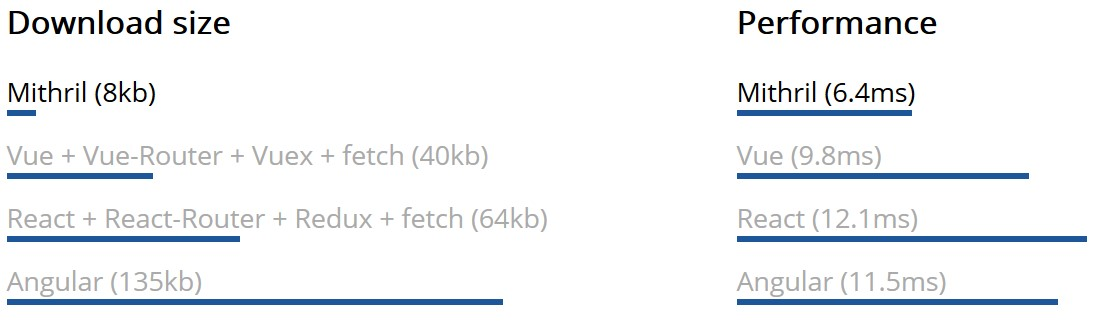
\includegraphics[width=14cm]{mithril-js-perf.jpg}
  \caption{Comparison of JavaScript frameworks size and performance\cite{mithril-speed}.}
  \label{fig:js-comp}
\end{figure}

\newpage
\section{Build system}
A corner stone in every project is the tool chain, it has to suit the use case and enhance the experience for the developers. A very common tool for managing JavaScript projects is NPM\footnote{Node Package Manager} which can acts as a build tool as well as package manager. In this scenario it will be used to lint and fix semantic issues found, manage dependencies, build the resulting JavaScript files and pack them with Webpack\cite{webpack}. NPM allows for freezing dependencies on specific version and also reports vulnerabilities when installing.

\section{Code editor}
The code editor was picked with the frontend language in mind. Since TypeScript originates from Microsoft, their web code editor Monaco, was implemented in this language, which led the developers to consider it an easier integration.
Apart from previously stated reasons, the Monaco editor (used in Visual Studio Code) has Microsoft Intellisense, syntax highlighting and auto completion among many advanced features.
The editor also benefits from using web workers, meaning that it can spawn a separate thread for the editor and not slow down the rest of the page.

The downside of using a hefty editor like this is the size. But by using lazy loading as explained in \autoref{sec:lazy-loading} this problem was mitigated.

\section{Graphing toolkit}
To generate graphs, a lightweight and simple tool with good community was premiered. D3.js was originally chosen but was quickly deemed too advanced for the simple visualizations used by the application. Chart.js is a simple, responsive and renders nicely on all platforms due to it using HTML5 canvas for rendering.

\section{Styling toolkit}
Styling can be a tedious task if done from scratch with pure CSS, to speed up development one can use a styling framework.
The frameworks considered were:

\begin{itemize}
    \item Bootstrap - widely used styling toolkit that both developers had experience with and therefore not chosen as learning something new was a course requirement.
    \item Semantic UI - simple syntax, predefined themes and ability to only load necessary stylesheets and JavaScript files which makes loading fast. This is the chosen framework.
\end{itemize}

Semantic UI also had support for customization using their \texttt{semantic-ui-less} package, this was used for customizing the search component.

\chapter{System architecture \& design}
\begin{figure}[H]
  \centering
  \includesvg[width=16cm]{architecture.svg}
  \caption{High level system architecture overview of the Roaster system.}
\end{figure}

\section{Infrastructure}
\begin{figure}[H]
  \centering
  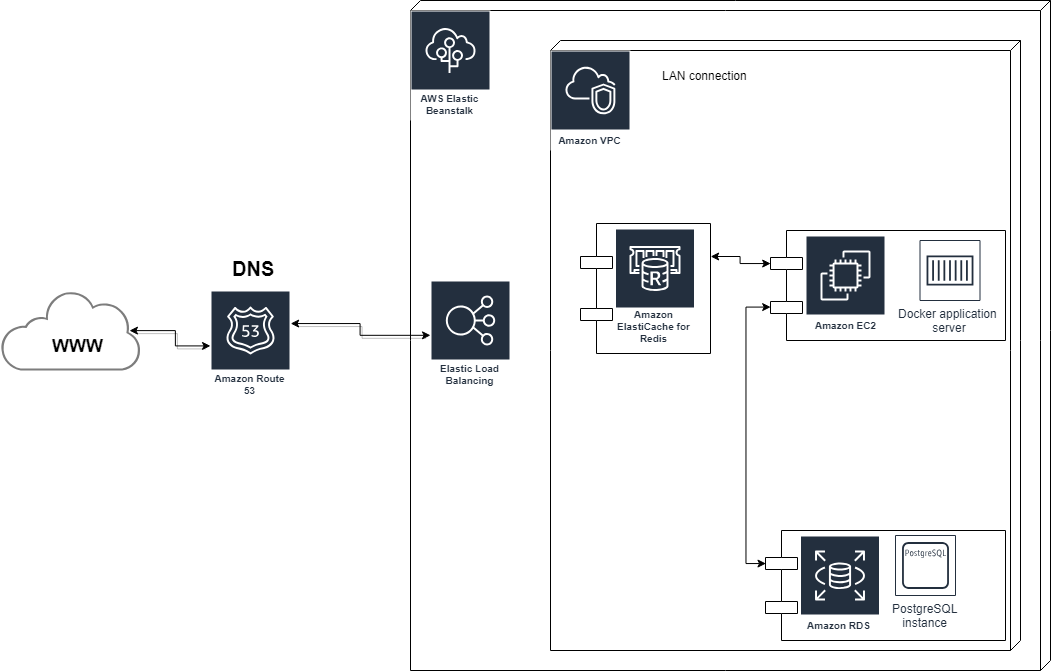
\includegraphics[width=16cm]{Cloud-infrastructure.png}
  \caption{AWS infrastructure.}
\end{figure}
The system is designed to be deployable independently without any dependencies to the  underlying platform. This led to containerization of the server in order to facilitate the deployment process and avoid installation mishaps. Both the databases are not containerized as these are run using AWS' SaaS\footnote{Software as a Service.} solutions instead.

The whole software architecture is designed to be scalable and is currently running on an Amazon Web Services (AWS) stack. PostgreSQL is used for persistent data storage and can be scaled accordingly depending on the usage requirements. The key store database Redis is used for shared user sessions between several web server instances. Like PostgreSQL, Redis can be scaled with database sharding and has support (through AWS) to run in several regions.

The web server (\texttt{roasterd}) runs in an Elastic Beanstalk (EB) environment that scales the web server automatically depending on the load. AWS uses nginx for load balancing which also provides certificates for HTTPS/TLS. Therefore, the web server behind the load balancer does not use HTTPS/TLS as it was deemed unnecessary.

If the solution is to be deployed at some other hosting solution like your own servers, and scalability is wanted, one would need to setup a load balancer in front of all the web servers. It's also wise to setup a heavily tested reverse proxy on the load balancer, like nginx. To match the size of your web servers you could also scale the databases. 

The communication between the application server and the databases are not encrypted as of now since they are all hosted in a Virtual Private Cloud (VPC) in AWS and thereby sandboxed. VPC also supports encrypted communication internally, but this is not used due to the cost. If implementing this on your own data centre or hardware you have to decide on this yourself in order to secure the architecture. The web server has  support for encrypted communication between both databases. 

\section{Web application (\texttt{roasterc})}
The web application design structure is based on the MVC\footnote{Model View Controller.} design pattern. To further isolate the logic the web application uses components, inspired by the pattern used by React\cite{react-component}. This is in-line with the reactive programming model that the Mithril.js framework is inspired by.

\subsection{SPA}
\begin{figure}[H]
  \centering
  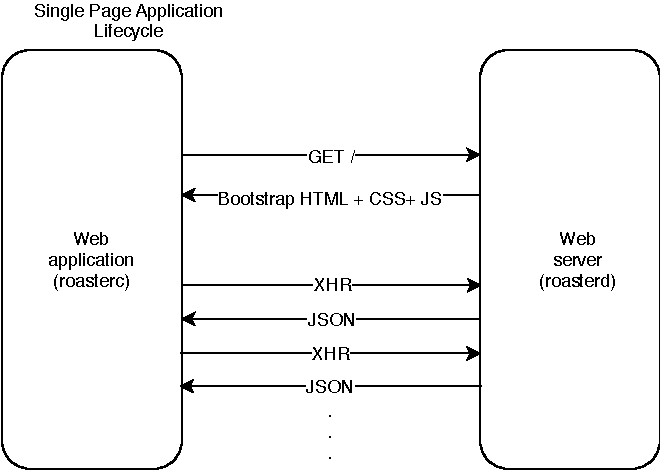
\includegraphics[width=10cm]{spa-lifecycle.pdf}
  \caption{Roasterc single page application lifecycle.}
  \label{fig:roasterc-lifecycle}
\end{figure}

The web application is a single page application (SPA) and is served as a single HTML document at the root (\texttt{/}) of the web server. The HTML document, CSS layouts and JavaScript files that is served through this endpoint bootstraps a client side router that serves each different view of the web application, see fig. \ref{fig:roasterc-lifecycle}. 

\begin{figure}[H]
  \centering
  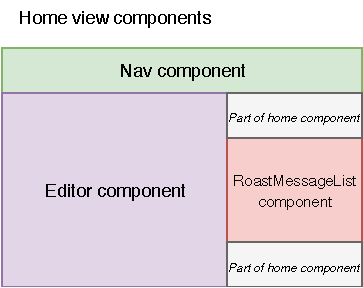
\includegraphics[width=10cm]{home-view-components.pdf}
  \caption{Example of components in the Home view.}
  \label{fig:home-view-components}
\end{figure}

These views are a collection of components each following the MVC pattern, see fig. \ref{fig:home-view-components}. Mithril.js allows the developer to create the views and components with Hyperscript that renders the HTML through the DOM\footnote{Document Object Model.}. The view is generated by diffing the current view with the new one, allowing Mithril.js to only update the relevant parts of the DOM. As a preliminary step to be able to do this fast, Mithril.js creates a \textit{Virtual DOM}, an internal representation of the DOM that it can work with faster.

\subsection{Asynchronous communication}
All communication that occurs with the web server except for the root endpoint is done RESTfully using the asynchronous XMLHttpRequest (XHR) API that is wrapped by Mithril.js and the web application as \texttt{Network.request}. The wrapping of the XHR API is due to the CSRF mitigation\footnote{Explained below in \autoref{subsec:csrf}}. Mithril.js will through this wrapper notify the Virtual DOM that it has to be updated after the network request has succeeded (or failed).

\subsection{Lazy loading}
\label{sec:lazy-loading}
The Monaco editor is used for code submission. It features code completion, highlighting and code mini maps. Even though large parts of the logic is handled in large web workers that runs in separate threads the main JavaScript file that is required is large. For a better user experience where a loading spinner is shown instead of a flickering HTML document it was decided that lazy loading of the editor was needed.

Therefore the Monaco editor is not linked with the initial HTML document. Instead, using Webpacks supports for using the \texttt{require() / import} call, the editor is loaded asynchronously and shown first when it has initialized the main components.

\section{Web server (\texttt{roasterd})}
Code reference/documentation for the \texttt{roasterd} web server (written in Go) can be found here: \url{https://godoc.org/github.com/LuleaUniversityOfTechnology/2018-project-roaster}.

\begin{figure}[H]
  \centering
  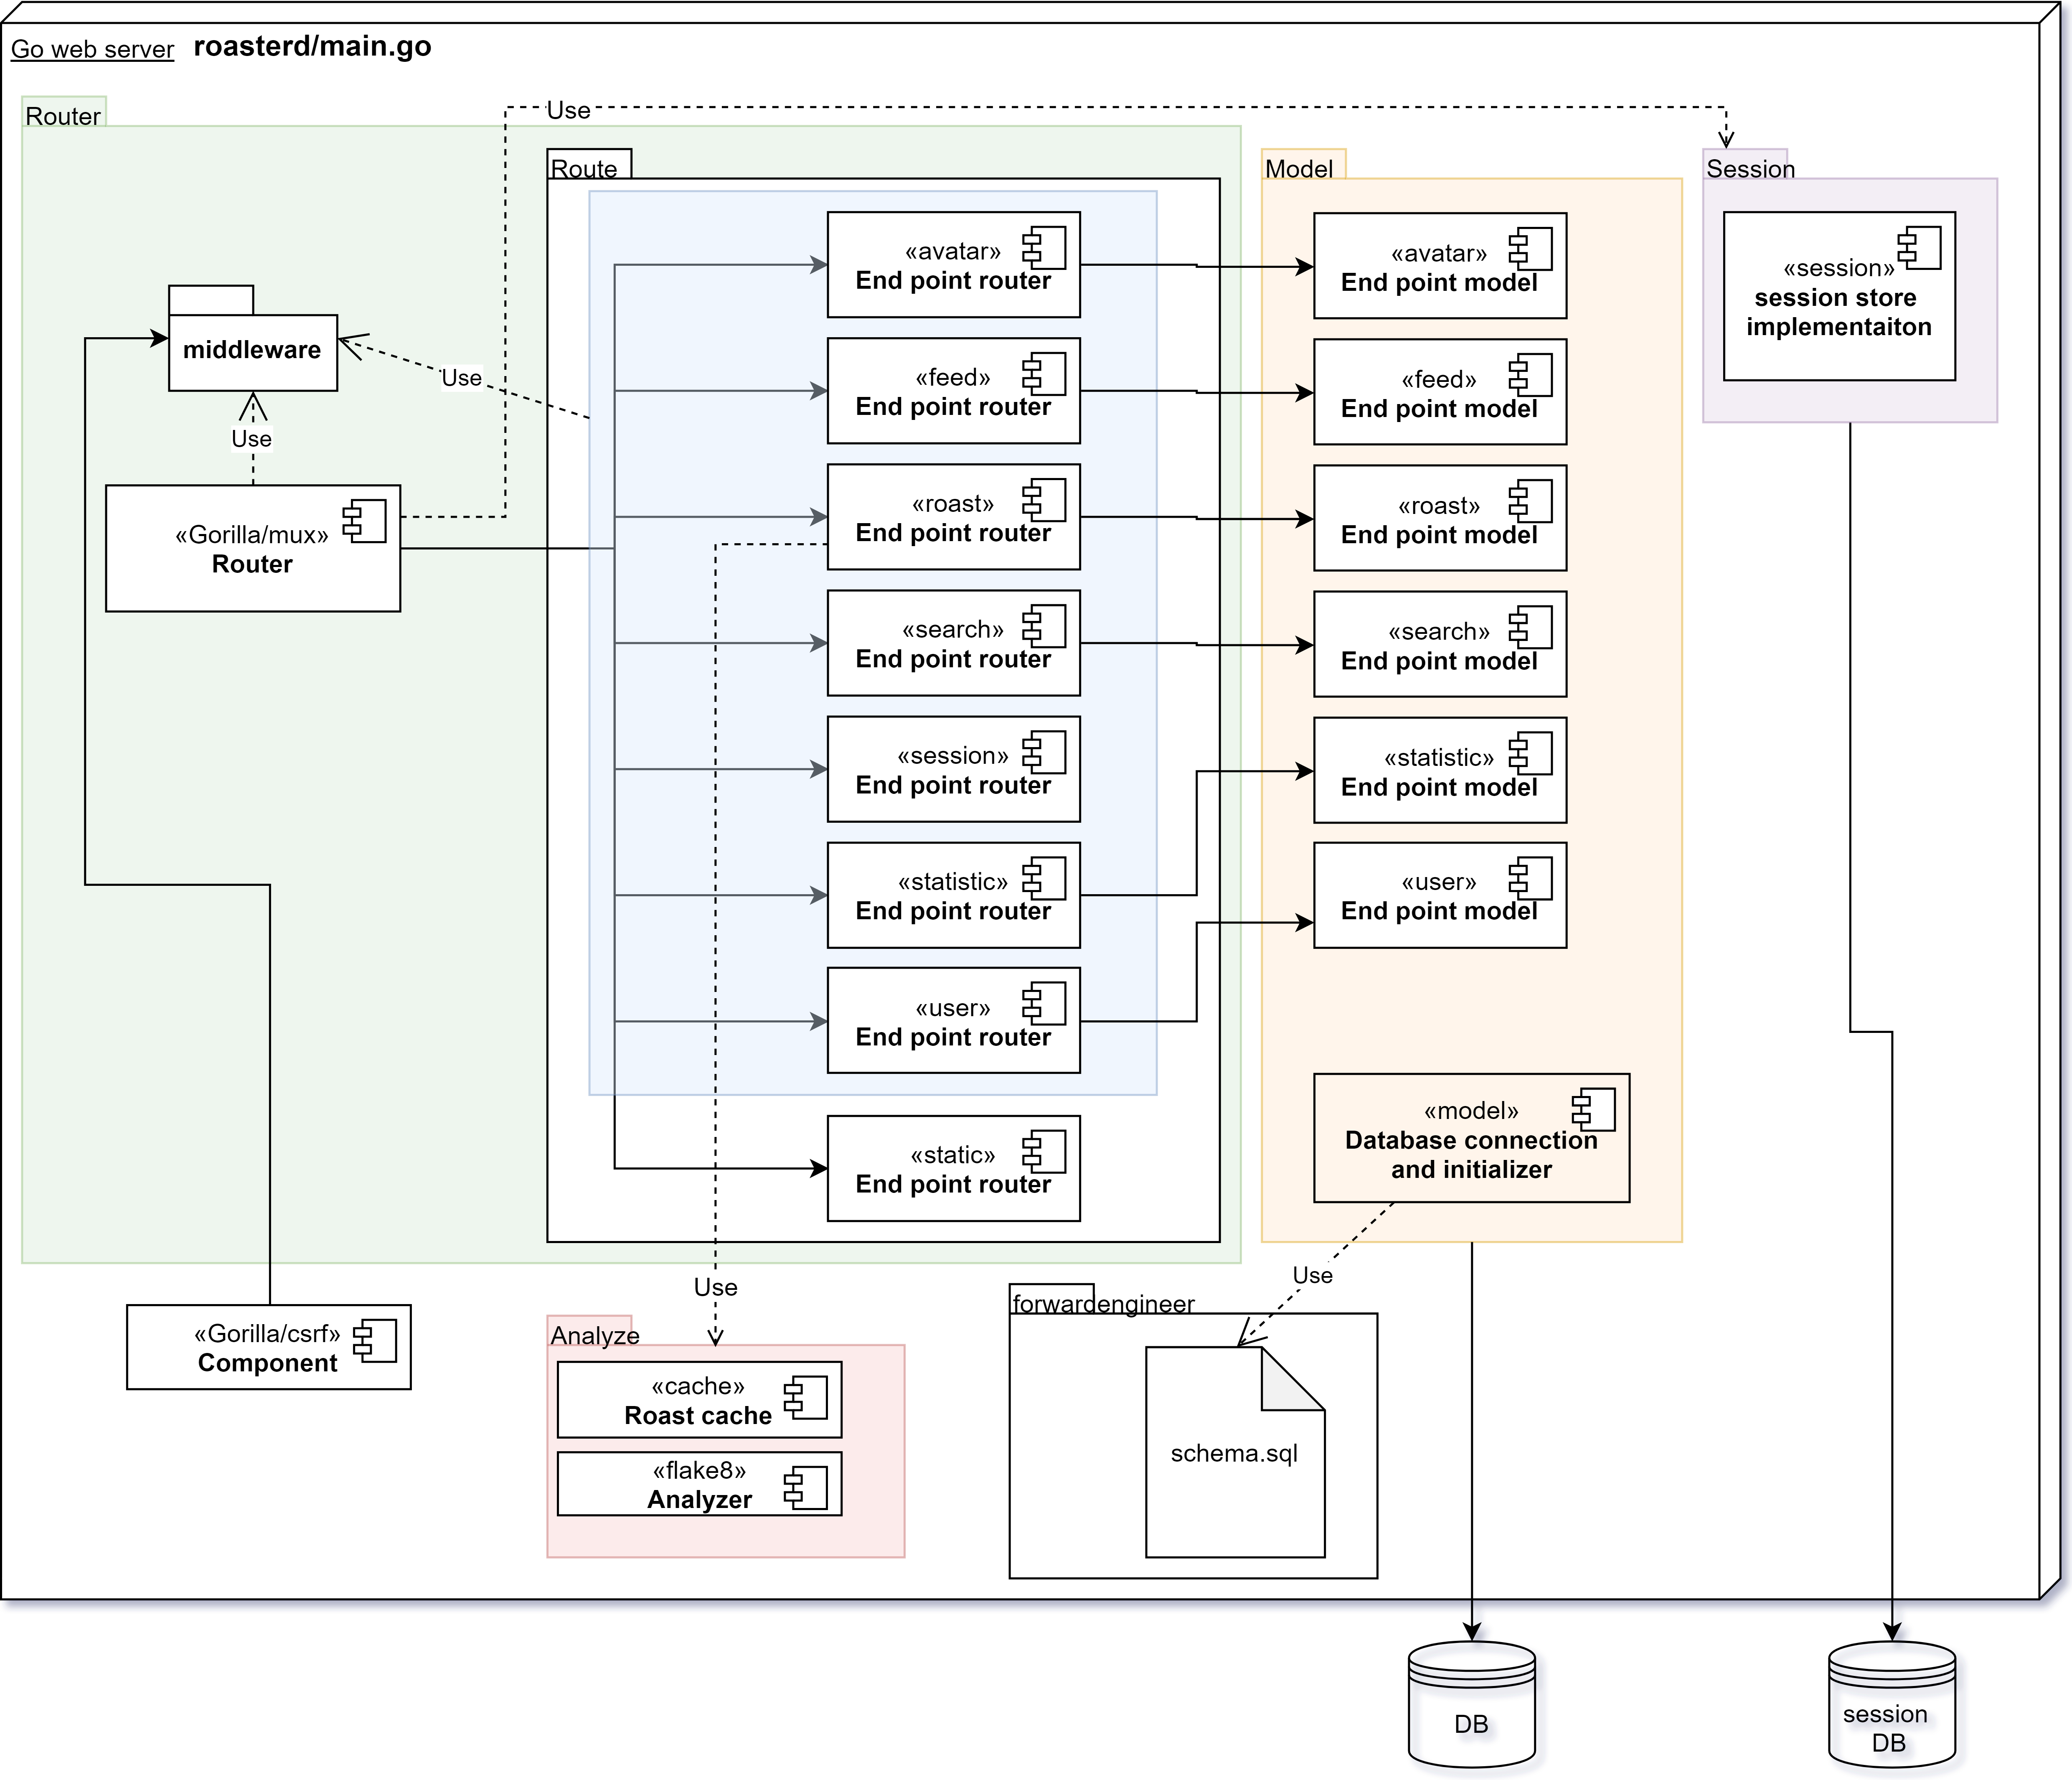
\includegraphics[width=17cm]{server-architecture.png}
  \caption{Web server (\texttt{roasterd}) architecture.}
\end{figure}

\subsection{HTTP and routing}
\begin{figure}[H]
  \centering
  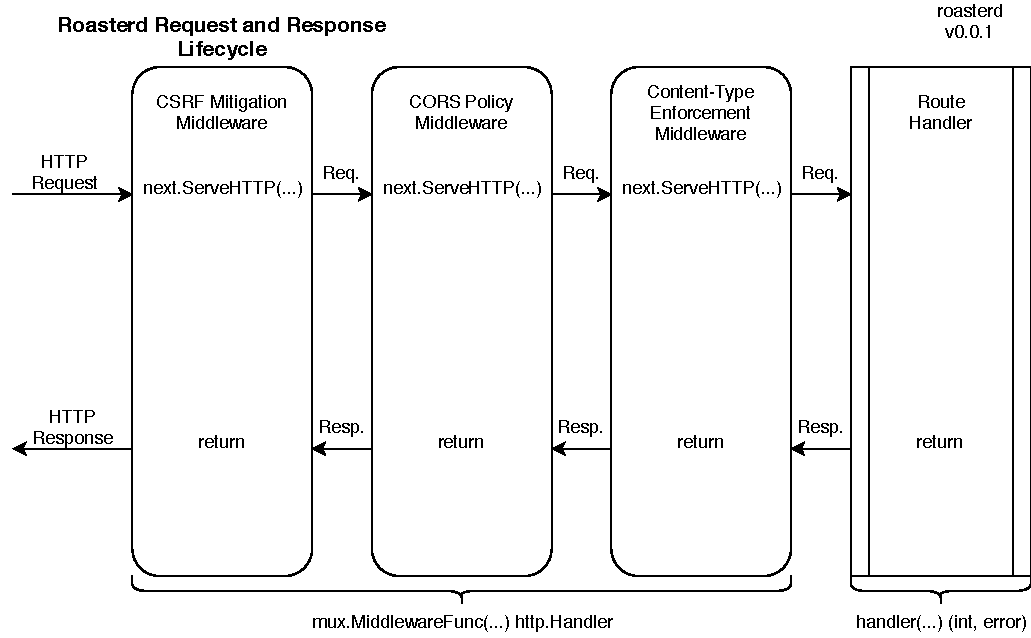
\includegraphics[width=16cm]{roasterd-req-resp-lifecycle-v0_0_1.pdf}
  \caption{Roasterd web server request and response lifecycle.}
  \label{fig:roasterd-lifecycle}
\end{figure}

Like the web application the web server is also based on the MVC design pattern. The generic handling of HTTP such as CSRF mitigation, \texttt{Content-Type} checking and CORS policies are implemented according to the middleware pattern. The middleware pattern abstracts parts into layers that are coupled together in a pipeline. At the end of the request chain the route handler that adheres to the MVC pattern handles the request and then sends a response that will go through the same middleware pipeline in the reverse direction, see fig. \ref{fig:roasterd-lifecycle}. The route handlers are defined in the \texttt{router/route}\cite{roaster-router-route} Go package and represents the controller and view in the MVC model. These route handlers talks to the database via the model that is contained in a separate Go package, called \texttt{model}\cite{roaster-model}.

\subsection{Analyzing code}
Static code analysis is used for grading submitted code. The \texttt{analyze} package implements the methods for each language. Currently only Python 3 is supported using the Flake8 suite and can be accessed through the \texttt{analyze.WithFlake8(...)}\cite{roasterd-analyze-withflake8} method. Any new languages that are added should provide their own \texttt{analyze.With...} method that follows the same interface as \texttt{analyze.WithFlake8}. The interface is defined as:
\begin{verbatim}
func(username, code string) (result *model.RoastResult, err error)
\end{verbatim}
Where \texttt{username} and \texttt{code} is the input and \texttt{result} and \texttt{err} is the output of the function.

The result from Flake8 is returned and encoded as JSON by the \texttt{flake8-json}\cite{flake8-json} formatter. The result is then unmarshalled into an unexported Go struct that follows the same structure as the JSON that \texttt{flake8-json} provides. This unexported struct is then converted into a \texttt{model.RoastResult} that can be saved to the database. The result is then returned to the callee, in this case the \texttt{/roast} route handler.

During development it was discovered that the Flake8 suite was very slow and took several seconds, even for small code snippets. The problem got even worse if a user decided to spam the API with code submissions - the web server would spawn several routines that all analyzed the same code snippet, resulting in a very simple DoS attack. To mitigate the easiest of attacks, and also increase the user experience with faster results, a simple cache was developed.

The cache can be found in the \texttt{analyze/cache}\cite{roasterd-cache} package and uses expiration and random replacement when it's filled.

\section{Database}
\begin{figure}[H]
  \centering
  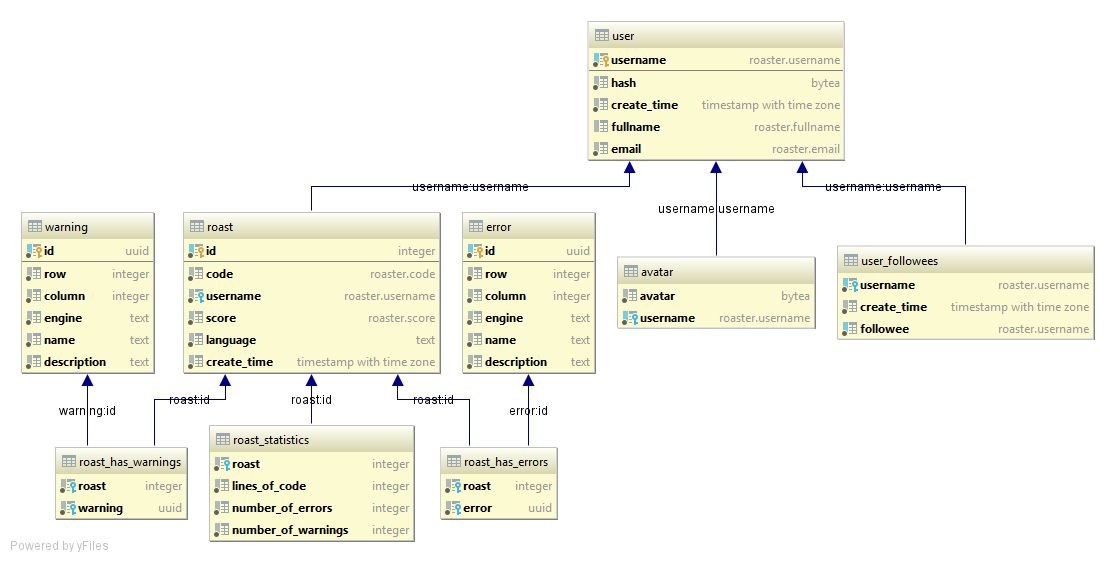
\includegraphics[width=16cm]{roaster-database-v0_0_1.png}
  \caption{UML diagram of the Roasterd SQL database design.}
  \label{fig:roasterd-database}
\end{figure}
PostgreSQL domains are utilized for validating the data stored in columns. This can be seen in fig. \ref{fig:roasterd-database} where the \texttt{username} column is of the type \texttt{roaster.username}. This custom domain data type will ensure that not any forbidden characters are in the usernames and that their length is atleast 3 characters and below 255. Similarly there are several other domains defined, such as \texttt{roaster.code}, \texttt{roaster.fullname} and \texttt{roaster.email}. The definitions for these domains can be found in \texttt{doc/postgresql/roaster-database-v0.0.2.sql}\cite{sql-def-line6}.

The same file also contains the whole definition of the SQL database used. This file is parsed by a program that can be found in \texttt{cmd/inlinesql}\cite{roasterd-cmd-inlinesql}. The program will copy each SQL statement into a Go slice (a type of array in Go) that can be used when the web server starts to bootstrap the database with the correct schema setup, this process is also known as \textit{forward engineering}.

\label{sec:database-messages}
The messages (errors and warnings for code submissions) are stored in separate tables using an UUID based on the content of the message as an identifier and primary key to prevent data duplication. Each message is then referenced by each submission result using a many-to-many relationship, e.g. between the \texttt{warning} table and \texttt{roast} table there is a table, \texttt{roast\_has\_warnings} that references each other. UUID is also supported as a data type in PostgreSQL\cite{pg-uuid} allowing for validating the UUID using their built-in constraints.

All user input from the API, except passwords, are validated against the database using its constraints instead of validating the data inside the web server's route handlers or model. This ensures that the actual data model is defined in one place and not spread out through out the application.

\section{API}
\label{sec:api-design}
The documentation for the Roaster REST API can be found at: \\ \url{https://roast.software/doc/restapi}.

The Roaster API is designed to adhere to the REST principles and at the same time be secure and support user sessions. A trade off has to be made for the requirement of being stateless in REST\cite{fielding-rest} where both the CSRF mitigation\footnote{Explained below in \autoref{subsec:csrf}.} and user session requires some state that is kept on the server-side. All API endpoints follow CRUD\footnote{Create, Read, Update, Delete} where the HTTP methods are used to represent each part, in the case of the Roaster API the following rules has been decided:
\begin{itemize}
    \item Create - \texttt{POST}
    \item Read - \texttt{GET / HEAD}
    \item Update - \texttt{PATCH / PUT}
    \item Delete - \texttt{DELETE}
\end{itemize}
The \texttt{PUT} method is used when a resource is overridden, such as when uploading a new profile picture. While the \texttt{PATCH} method is used when the request have the feature of replacing partial data, such as when updating partial user profile information. \texttt{POST} is used when a new resource should be created, such as a new code submission. The \texttt{DELETE} method is used for e.g. removing an user that you are following. The \texttt{GET} and \texttt{HEAD} method should never modify any data.

The Roaster API tries to use clean and logical URI components. The structure uses URI components as categories that are routed to sub-routers in the backend. An example is the \texttt{/user} route, which has several endpoints such as
\begin{itemize}
    \item \texttt{/user/\{username\}} - User profile information handling for \textit{\{username\}},
    \item \texttt{/user/\{username\}/avatar} - Change or retrieve profile picture for \textit{\{username\}},
    \item \texttt{/user/\{username\}/followers} - Retrieve a list of followers for \textit{\{username\}}.
\end{itemize}
Where the \texttt{/user} sub-router dispatches different handlers depending on the last URI component (e.g. \texttt{/avatar} or \texttt{/followers}) together with the username as a parameter. In the case of \texttt{/user/\{username\}} the sub-router sees the last URI component as \texttt{/}.

The HTTP status codes are used to denote both different successful states and error states. The \texttt{200 - OK} code is returned if the request was successful and there is data to return. While \texttt{204 - No Content} is used when there is no data to return, e.g. after updating a profile picture or when the user has no followers. The status codes can be found in the REST API documentation mentioned above.

\newcommand{\rratio}{Roast\textsuperscript{\textregistered} Ratio\textsuperscript{\texttrademark}}
\newcommand{\rscore}{Roast\textsuperscript{\textregistered} Score\textsuperscript{\texttrademark}}

\section{Grade system}
There are two different simple measurements for the submitted code, \rscore and \rratio.

The \rscore is calculated per code submission and is defined as follows:
\begin{equation*}
    \text{\rscore} = \left\lfloor\frac{L}{0,8E + 0,29W + 1}\right\rceil
\end{equation*}
Where $L$ is the number of lines of code and $E$ and $W$ is the number of errors and warnings, respectively. The cost set for an error is $0,8$ and $0,2$ for a warning, so for every line of code $0,8$ points is removed if it's an error and $0,2$ is removed if it's a warning. So a line with both an error and a warning is worth $0$ points. The resulting score is rounded to the nearest integer. The \rscore can never be less than $0$.

The \rratio can be calculated for both single submissions or all, it's defined as:
\begin{equation*}
    \text{\rratio} = \left\lfloor 1 - \frac{E + W}{S} * 100 \right\rceil
\end{equation*}
Where $S$ is the number of \textit{successful} lines, i.e. line without any errors or warnings. $E$ and $W$ is as previous the number of errors and warnings. The \rratio formula will return a percentage where $100 \%$ is the best possible ratio.

%\chapter{System architecture}
% Move to security section, I wrote some stuff about this in the chapter above, too
% The flake8 component that analyzes Python code is executed in the same docker container as the application server. This is safe since the flake8 analyzer does not run any code, only parses it.
% The application server has access to local system calls and can thereby start the analyzer. The communication back from the analyzer is encoded in JSON which is very convenient to work with in Go due to the well developed JSON library in Go.


% Same as above?
% The frontend is based on a JavaScript framework called Mithril.js that encourages modularization and a model component based pattern. This takes advantage of a virtual DOM that utilizes diffing which makes it very fast, and mitigates many security risks like XSS attacks. 

\chapter{API}
The Roaster API v0.0.1 is fully documented and can be viewed at the following address: \url{https://roast.software/doc/restapi/}. The API tries to adhere to the REST principles and is designed around the CRUD pattern, see \autoref{sec:api-design} for more information.

\section{Bootstrap with CSRF mitigation}
\label{sec:api-bootstrap}
All API endpoints are protected with CSRF mitigation, except for \texttt{GET, HEAD, OPTIONS} and \texttt{TRACE} (non-write operations). Therefore before doing write operations such as \texttt{POST} and \texttt{PUT} the \texttt{X-CSRF-Token} has to be retrieved. Even if \texttt{GET} isn't protected with CSRF mitigation the web server will respond with a fresh \texttt{X-CSRF-Token} that can be used for doing a write operation.

A simple \texttt{HEAD} request to the \texttt{/} endpoint will give all the headers that the web server would respond with for a \texttt{GET} request. This is utilized to only retrieve the required token and not the whole web application that it would normally do.

In the following example cURL is used to demonstrate the bootstrapping process.

First, retrieve the \texttt{X-CSRF-Token} header and the CSRF challenge cookie with:
\begin{verbatim}
curl -c cookies.txt --head https://roast.software/ \
    | grep -Fi x-csrf-token > token.txt
\end{verbatim}
Where \texttt{cookies.txt} contains the cookies and \texttt{token.txt} contains the next \texttt{X-CSRF-Token}.
The \texttt{cookies.txt} and \texttt{token.txt} files can be read by specifying \texttt{-b cookies.txt -H @token.txt} as arguments to cURL.

\newpage
For any following request that is a write operation the cookies and token has to be sent by the client, for a \texttt{POST /roast} the command would be:
\begin{verbatim}
# -i - Include response headers in output.
# -b cookies.txt - Read the cookies (incl. challenge).
# -c cookies.txt - Write the new cookies (incl. challenge).
# -H @token.txt  - Read token.
curl \
    -b cookies.txt \
    -c cookies.txt \
    -H @token.txt \
    -H "Content-Type: application/json" \
    -X POST https://roast.software/roast -d \
    "{ \
        \"language\": \"python3\", \
        \"code\": \"print('Hello, world!')\" \
    }"
\end{verbatim}

\section{Authenticate an user}
Because the authentication towards the API is a \texttt{POST} request the CSRF mitigation has to be bootstrapped as explained in \autoref{sec:api-bootstrap}. After the bootstrapping has been done the following API request will authenticate a user and save the resulting session cookie:
\begin{verbatim}
curl \
    -b cookies.txt \
    -c cookies.txt \
    -H @token.txt \
    -H "Content-Type: application/json" \
    -X POST https://roast.software/session -d \
    "{ \
        \"username\": \"willeponken\", \
        \"password\": \"my_very_secure_password\" \
    }"
\end{verbatim}

Now any endpoint that requires a session can be queried, e.g. modifying the user profile information:
\begin{verbatim}
curl \
    -b cookies.txt \
    -c cookies.txt \
    -H @token.txt \
    -H "Content-Type: application/json" \
    -X PATCH https://roast.software/session -d \
    "{ \
        \"email\": \"mail@example.org\", \
        \"fullname\": \"William von Willeponken\" \
    }"
\end{verbatim}

% \chapter{Description of software parts and interaction between them}

\newpage

\chapter{Security considerations}
Several security issues has been taken into consideration when developing the system. The OWASP Top 10 list\cite{owasp-top-10} has acted as a reference during the project to decide what security problems to prioritize and look for.

\section{HTTPS/TLS}
The connection from the client to the web server is made over TLS with a Amazon signed certificate.
This is configured by the Elastic Load Balancer running on Elastic Beanstalk that acts like a reverse proxy.
The request then propagates through the VPC (Virtual Private Cloud) in AWS in plaintext. 

\section{Injection}
Injection was the top security vulnerability in OWASP Top 10 list\cite{owasp-top-10}. For Roaster this includes SQL and OS injections. Go's \texttt{database/sql} library enforces SQL parameterization per default with placeholder parameters\cite{go-database-sql}, ensuring that SQL injections are not possible, as the values are binary safe. OS injections could be an issue due to that the analyzis of code is passed to a separate OS level process (in this case the Python 3 application Flake8). This issue is solved by not allowing any change of the actual command that gets passed to the OS - it's hard coded and only allows for input through a Linux pipe. Flake8 also does not execute any of the code that it analyzes as the program only uses static code analysis\cite{pyflakes}\cite{mccabe}\cite{pycodestyle}.

\section{CSRF}
\label{subsec:csrf}
The site has implemented protection against CSRF (Cross Site Request Forgery). CSRF is a man-in-the-middle attack where the automatic cookie submission\footnote{The cookie is always sent for every request by the web browser.} is abused. A site that utilizes cross-origin requests cannot use the \texttt{site-only} attribute for cookies, i.e. another malicious website open in another tab can also issue authenticated requests to the web service\cite{rick}. The CSRF security risk was downgraded on the OWASP Top 10 because most frameworks implement and enforce mitigations per default\cite{owasp-top-10}, but because the system is written without any framework this has to be implemented manually.

In order to increase the security against CSRF attacks a rolling random token scheme was chosen and implemented. The rolling scheme ensures that the CSRF token is not stolen as demonstrated by the BREACH attack\cite{breach}. First, a CSRF cookie is issued by the web server to sign challenges against, then a challenge is issued by the web server as a HTTP header called \texttt{X-CSRF-Token} for every request.

A custom network handling system had to be implemented that wraps XHR requests in the frontend due to the CSRF mitigation system.  The library that has been implemented, called \texttt{Network}\cite{roaster-network}, wraps the Mithril.js \texttt{m.request} method and retrieves the new \texttt{X-CSRF-Token} header for every requests and then saves it so it can be used for the next XHR request.

All HTTP methods, except \texttt{GET, HEAD, OPTIONS} and \texttt{TRACE}, that are sent to the web server are required to authenticate with the CSRF challenge response mechanism. Therefore the \texttt{Network} library creates a \texttt{HEAD} request toward the \texttt{/} (root) API endpoint to receive the first initial \texttt{X-CSRF-Token} for the rolling scheme.

Cookie security that can mitigate XSS attacks is discussed below in \autoref{subsec:secure-cookies}.

\section{XSS}
The Mithril.js framework will automatically escape all HTML tag characters before inserting into the Virtual DOM that it creates\cite{mithril-trust}. Therefore most XSS (Cross Site Scripting) issues are mitigated. However, because jQuery is used for the search component extra caution has to be taken. The jQuery Search plugin \textit{does not} escape HTML tag characters so in this case the escaping has to be done explicitly.

Removing the jQuery dependency is discussed in \autoref{subsec:remove-jquery}.

Cookie security that can mitigate XSS attacks is discussed below in \autoref{subsec:secure-cookies}.

\section{Secure cookies}
\label{subsec:secure-cookies}
User session cookies is stored in the cookie store in the browser. These are validated with the HMAC verification mechanism and encrypted with AES-256. HMAC verification ensures that the cookie content has not been tampered with during the transfer\cite{fips-198}. While AES-256 encrypts the data contained within the cookie, ensuring that no one can read it\cite{fips-197}. Even with TLS these are real issues due to the BREACH/CRIME vulnerability that is able to extract the HTTP headers for encrypted transfers\cite{breach}. The BREACH attack is mitigated using the rolling CSRF token scheme explained in \autoref{subsec:csrf}.

The session cookies has the \texttt{HttpOnly} attribute enabled which sandboxes the cookie so it cannot be accessed by JavaScript. This will mitigate the most common XSS attacks\cite{owasp-httponly}. Additionally the \texttt{sameSite} attribute is set to \texttt{Strict} which tells the browser that it should not send the cookie with cross-site requests\cite{owasp-samesite}. The \texttt{sameSite} attribute will mitigate CSRF attacks, but is only supported in modern browsers. As of August 2018 only $68,92 \%$ of the browsers used by Internet users supports the \texttt{sameSite} attribute\cite{owasp-samesite-support}. It was concluded that this low adoption is reason enough to implement the rolling CSRF token scheme described above.

\section{Password storage}
There are a lot of challenges keeping user credentials secured. The solution that was chosen is based on well known algorithms, Bcrypt and SHA-512. The implementation uses official libraries in Go, the language in which the server is written.

The plaintext password that is provided by the user will first be transformed to a hash sum with SHA-512. This is due to that Bcrypt limits the input to 72 bytes. By hashing the password with SHA-512 more entropy of the original password is kept. Also, some implementations of Bcrypt that allows for longer passwords can be vulnerable to DoS attacks\cite{bcrypt-length}.

The SHA-512 hash sum is then hashed again using Bcrypt. This is because
SHA-512 is a \textit{fast} hash algorithm not made for password hashing. Bcrypt is
designed to be slow and hard to speed up using hardware such as FPGAs and
ASICs. The work factor is set to 12 which should make the expensive Blowfish
setup take $> 250$ ms\footnote{$364.815906$ ms precisely on one of the developers slow laptop.}.
The Bcrypt algorithm also takes care of salting of the password and prepends 
it with the resulting hash.


Dropbox has a great article\cite{dropbox-passwords} on their password hashing scheme
which the Roaster scheme shares many similarities with, however, encryption using AES-256
with a global pepper\footnote{Shared global encryption key.} is not used. This was deemed overkill 
by the developers for the use case of this project. Dropbox also encodes their SHA-512 with base 64,
which is not needed in the case of Roaster because the hash result can be saved as raw
bytes\footnote{Using PostgreSQL's \texttt{bytea} data type.}.

Some implementations of Bcrypt uses a null byte (\texttt{0x00}) to determine the end
of the input\cite{bcrypt-bug}, the Go implementations does \textit{not} have this problem. So there
is no need to encode the data as base 64. This is verified using the program that was created for
this project in the \texttt{cmd/testbcrypt} source folder.

The approach used by Dropbox where they encode with base $64$ will generate a
$\approx 88$ byte long key, which is then truncated to $72$ bytes. This results in a
input with $64^{72}$ possible combinations. The Roaster approach of not encoding the
input as base $64$ results in a $64$ byte long key\footnote{The output size of SHA-512.},
where there is 256 possible combinations \textit{per byte}. This results in an input
with $256^{64}$ possible combinations. Therefore the Roaster approach allows for far more
possible entropy because $64^{72} \ll 256^{64}$ ($\approx 1,2 \times 10^{24}$ times more!).

The amount of possible entropy for both solution is so high that comparing the differences
between them two doesn't really make sense - but the Roaster solution that allows for more entropy
\textit{also} skips the unnecessary base 64 encode step due to the lack of the null byte bug.

The only requirements set for passwords are a minimum length of 8 characters and a maximum of 4096 characters. The reason is that too many password rules, such as requiring specific characters, will lower the available entropy of the password. Also, with too strict requirements the users usually picks easy to guess patterns, like using \texttt{!} or \texttt{1} at the end of the password due to requirements of special characters and numbers\cite{oauth-nist}. NIST\footnote{National Institute of Standards and Technology in the US.} publishes guidelines for password handling each year. In addition to the password length requirement they also recommend 2FA\footnote{Two Factor Authentication}\cite{nist-passwords}. This is not yet implemented but would be a future improvement of the security.

\chapter{Discussion}

\section{Cloud provider}
In hindsight, the team might have chose a different cloud provider due to complexity in the configuration and maintaining of the service. The cost model is elusive which causes unnecessary re-configurations when choosing a too (cost) expensive configuration. The re-configurations wouldn't be such a problem if it were a more streamlined process and a matter of adjusting a few things in the web interface rather than rebuilding the majority of the environment, which could take hours. The documentation is decent but gives more to ask for when something is not behaving like expected, this made the developers having to resort to unofficial sources for debugging the environment. The logging of the environment could also be better, only outputting logs with scrambled time stamps makes it very hard to read. A cloud provider which offers a simpler service would suffice until the architecture of the site becomes more complex like wanting to run the Python code analyzers as micro services etc.

\section{Mithril.js}
Mithril.js has been a challenge to work with, accidentally using the documentation for version 2 of Mithril.js whilst actually using Mitril.js version 1. The documentation available is also sparse and not very exhaustive. The community is still small compared to the framework giants like React.js, Angular.js and Vue.js which makes finding good examples that describe advanced maneuvers a lot harder. The source code also has a high grade of coupling that makes modifications to it's inner workings problematic. As an example the developers wanted to extract the CSRF token on XHR responses, but \texttt{m.request} that was provided by Mithril.js skipped the JSON parsing and error handling if the developer provided their own \textit{extract} function. Due to the too high coupling in the Mithril.js implementation it was not possible to re-use their own logic and the developers had to re-implement the same functionality themselves.

The design pattern with components that is enforced by the framework was clearly document when writing untyped JavaScript code. However, the examples for writing the same code with typed TypeScript was either missing or was written in an experimental style that the authors of the framework tried. This led the developers to also try several different code styles during the project. Several of these style can still be found in the project, some with lower readability. The developers are still unsure what style to use, but no matter what, a re-factoring of several components, views and models is required.

\section{Semantic UI}
With the experiences gained from Semantic UI, the developers are not so sure they would use it again. This is mainly due to the dependency on jQuery for certain common features like the search bar. jQuery as a technology does not escape HTML per default\cite{jquery-sucks} and will introduce a whole new plethora of attack vectors for injection and scripting attacks. Everything that can be done with jQuery can also be accomplished with JavaScript/TypeScript and is therefore considered an unnecessary risk by the developers.

If the project site were to be re-designed, then the developers would most probably choose another CSS framework like Materialize, Milligram or Foundation depending on what would be prioritized in the next version of the site. Materialize\cite{materialize} for a fast remake, Milligram\cite{milligram} for mobile focused design and Foundation\cite{foundation} for an uncompromising design which can offer Graphics Proccessing Unit accelerated animations, and mobile specific elements for fast experience on a mobile device.

\section{Editor}
The Monaco editor was chosen partly because of it being written in TypeScript and was thought to ease integration into the web application. One of the serious alternatives was the CodeMirror editor\cite{codemirror}, but was at the time of choosing technologies, not written in TypeScript. During the time of developing Roaster CodeMirror has gone through a rewrite and there is now an unreleased version based on TypeScript\cite{codemirror-ts}. One of the goals of the site was to make it feel fast and responsible, once loaded the site achieves these goals with flying colors but the developers would in hindsight prefer a smaller editor with less features. Many features used in Monaco are left disabled, such as the mini map.

Another alternative than moving to CodeMirror would be to optimize the Webpack compilation so the Monaco editor would be better separated into smaller JavaScript chunks. Some optimization has already been done, but there is a possibility that it can be improved further.

\chapter{Future work}
\label{sec:future-work}
The proof of concept is finished for Roaster and the service works as we wanted, but there are several ways to extend the service and improve it. Below follows some larger changes that could extend Roaster. Additionally the current issues that should be solved before extending Roaster is presented in \autoref{sec:issue-tracker}.

\section{More languages}
One of the more obvious improvements is to add more languages than Python 3. A simple start would be to add Python 2.7. An interface for each language's static analyze toolkit has to be implemented that can fulfill the \texttt{analyze/...} package's generic \texttt{RoastResult} interface. Adding other languages than Python should be easy, but requires that a new toolchain and environment is setup for that specific language on the same system as the web service is running.

\section{Microservices}
To ensure that the service can scale as it grows the analyze system could be split into separate microservices for every language. Even in its current implementation a cache is required due to the slowness of the static analysis tools. Microservices would greatly reduce the load on the main web services. The microservice would communicate using a message queuing system, e.g. RabbitMQ, where the main web services can publish a new request and get a response later from one of the microservices. These microservices would be easy to scale for user demand.

\section{Statistics}
The presentation and collection of statistics could need more work so that more relevant statistics is presented to the user. An easy start would be statistics for the type of errors and warnings - the data already exists in the backend but is not compiled together for easy parsing through the REST API.

\section{CLI \& IDE integration}
One feature that the developers had in mind from the start was integrating the system with a CLI tool and IDE's. Developers could hook their development environment with a CLI that will automatically send their code, on save or commit, to Roaster using its REST API. The API is already built to be easy to integrate with and it should be trivial to create a simple CLI tool. Integrating Roaster with IDE's would allow the score and statistics to be displayed directly inside the IDE, and at the same time allow for the coders friends to view their progress through the Roaster web interface.

\section{Refactor frontend components}
As mentioned in the discussion a refactoring of the components is required for some components in the frontend source. There is no clear set code style that has been chosen by the developers and this would require further pre-studying before refactoring.

% Vi kan nog skippa detta sålänge, kanske lägga till ifall Parnes vill ha mer idéer till framtiden.
% \todo{Maybe write some about the idea around analyzing whole projects with multiple files folders? Could a future improve ment be to be able to upload a zip file to roaster web interfacE?}

\section{Enhanced security}
Currently only passwords are supported as authentication. One improvement would be 2FA, Two Factor Authentication, this is recommended by NIST in their password handling \\ guidelines\cite{nist-passwords}. There are many other security measures that could be implemented that is mentioned in the guidelines. A \textit{Show Password} button and password blacklisting are two simple improvements mentioned\cite{oauth-nist}.

\newpage
\section{Issue tracker}
\label{sec:issue-tracker}
\textbf{\textsuperscript{F}} Requires frontend changes. \\
\textbf{\textsuperscript{B}} Requires backend changes.

\subsection*{Enhancements}
\subsubsection{Remove jQuery\texorpdfstring{\textsuperscript{F}}{}}
\label{subsec:remove-jquery}
jQuery is used for the search feature and was added due to time constraints, in the future the search component can be implemented with Mithril.js and the jQuery dependency can be removed, thus removing the overhead of having to mitigate XSS injections for non-Mithril.js components.

Tracked in issue: \href{https://github.com/LuleaUniversityOfTechnology/2018-project-roaster/issues/225}{\#225}

\subsubsection{Refactor UserModel\texorpdfstring{\textsuperscript{F}}{}}
The logged in user's data is saved in the static \texttt{UserModel} model. It would be better to have a object that is passed to the views that require them (composition), this would allow for merging the \texttt{Profile} and \texttt{User} views for more DRY\cite{dry} code. Additionally the request methods should be moved into the model to prevent code duplication. The statistics models are already implemented like this and can be used as insperation.

Tracked in issue: \href{https://github.com/LuleaUniversityOfTechnology/2018-project-roaster/issues/184}{\#184}

\subsubsection{Use LESS instead of overriding CSS through Mithril.js\texorpdfstring{\textsuperscript{F}}{}}
The Semantic UI styling framework is used for most of the styling of the views. In some cases the definitions by Semantic UI is overrided inline through Mithril.js. Later during the project the \texttt{semantic-ui-less} package was pulled in and integrated with the Webpack build environment. Most of the inline CSS definitions can be removed and be defined as LESS that is compiled together with Semantic UI instead.

Tracked in issue: \href{https://github.com/LuleaUniversityOfTechnology/2018-project-roaster/issues/130}{\#130}

\subsubsection{Clean up error handling\texorpdfstring{\textsuperscript{F}}{}}
There is no clear error handling pattern used for the frontend. The situation has gotten better throughout the project but there are still some parts of the code base that do not handle errors in a nice way.

Tracked in issue: \href{https://github.com/LuleaUniversityOfTechnology/2018-project-roaster/issues/115}{\#115}

\subsection*{Features}
\subsubsection{View specific Roast result\texorpdfstring{\textsuperscript{F+B}}{}}
After a user has been Roasted their submission is saved in the database, but they cannot view their code later when they have closed the page. A feature where they can view their previous results would be a great addition to view their progress.

This would require us to implement new API endpoints and also create a new view with the Monaco editor.

Tracked in issue: \href{https://github.com/LuleaUniversityOfTechnology/2018-project-roaster/issues/163}{\#163}

\subsection*{Bugs}
\subsubsection{Fix overflow for Roast submission messages\texorpdfstring{\textsuperscript{F}}{}}
There is an issue where the scrollbar doesn't appear when the Roast submission messages overflow. This happens when the user submits code with many errors and/or warnings.

Tracked in issue: \href{https://github.com/LuleaUniversityOfTechnology/2018-project-roaster/issues/134}{\#134}

\subsubsection{Register XHR request callback gets interrupted by Google  Chrome\texorpdfstring{\textsuperscript{F}}{}}
With a cold browser cache the XHR request callback gets interrupted by Google Chrome. This is \textit{probably} due to the 6 max TCP connections limit in the web browser. This bug only occurs for Google Chrome with a cold cache, if the cache is warm there is no issues.

The interrupt will stop Mithril.js from redirecting to the front page upon a successful registration. The user registration is correctly registered by the backend and the user is still able to login with the newly created account.

Tracked in issue: \href{https://github.com/LuleaUniversityOfTechnology/2018-project-roaster/issues/226}{\#226}

\subsubsection{Requirement for full name differs with the backend\texorpdfstring{\textsuperscript{F}}{}}
Upon registration the user is required to fill in their full name, even though it's not a requirement in the backend. Several views in the frontend utilizes the full name and they should be updated to show the username if there is not full name defined.

The registration requirement for a full name can be removed after the views has been updated.

Tracked in issue: \href{https://github.com/LuleaUniversityOfTechnology/2018-project-roaster/issues/210}{\#210}

\newpage
\apptocmd{\sloppy}{\hbadness 10000\relax}{}{} 
{\RaggedRight\begin{thebibliography}{1}

\bibitem{rick}
Ramgattie, R (2018, May 14) {\em  Cracking Java’s RNG for CSRF - Javax Faces and Why CSRF Token Randomness Matters.}
Fetched 2019-01-10, from:
\url{https://blog.securityevaluators.com/cracking-javas-rng-for-csrf-ea9cacd231d2}.

\bibitem{breach}
Gluck, Y., Harris N., \& Prado A. (2013, July 12) {\em BREACH: Reviving the Crime Attack, pp. 3, 11.} \\
Fetched 2019-01-10, from:
\url{http://breachattack.com/resources/BREACH\%20-\%20SSL,\%20gone\%20in\%2030\%20seconds.pdf}.

\bibitem{roaster-network}
LuleaUniversityOfTechnology/2018-project-roaster (2019) {\em 2018-project-roaster/network.ts at 19529..28560.}
Fetched 2019-01-10, from:
\url{https://github.com/LuleaUniversityOfTechnology/2018-project-roaster/blob/1952964/www/src/services/network.ts#L38}.

\bibitem{mithril-trust}
Mithril.js 2.0.0-rc3 (2018) {\em trust(html) - Mithril.js}
Fetched 2019-01-10, from:
\url{https://mithril.js.org/trust.html#how-it-works}.

\bibitem{fips-198}
NIST (2002, March 2) {\em FIPS 198-1, The Keyed-Hash Message Authentication Code (HMAC), p. 1.} \\
Fetched 2019-01-10, from:
\url{https://ia902804.us.archive.org/2/items/DTIC_ADA401868/DTIC_ADA401868.pdf}.

\bibitem{fips-197}
NIST (2001, November 26) {\em FIPS 197, Annoucing the Advanced Encryption Standard (AES), p. 5.} \\
Fetched 2019-01-10, from:
\url{https://ia802809.us.archive.org/0/items/DTIC_ADA403903/DTIC_ADA403903.pdf}.

\bibitem{owasp-httponly}
OWASP (2017) {\em HttpOnly.} Fetched 2019-01-11, from:
\url{https://www.owasp.org/index.php/HttpOnly}.

\bibitem{owasp-samesite}
OWASP (2017) {\em SameSite.} Fetched 2019-01-11, from:
\url{https://www.owasp.org/index.php/SameSite}.

\bibitem{owasp-samesite-support}
OWASP (2017) {\em Cross-Site Request Forgery (CSRF) Prevention Cheat Sheet.} Fetched 2019-01-11, from:
\url{https://www.owasp.org/index.php/Cross-Site_Request_Forgery_(CSRF)_Prevention_Cheat_Sheet#Samesite_Cookie_Attribute}.

\bibitem{owasp-top-10}
OWASP (2017) {\em OWASP Top 10 - 2017, pp. 4, 6.} Fetched 2019-01-16, from: \url{https://www.owasp.org/images/7/72/OWASP_Top_10-2017_\%28en\%29.pdf.pdf}.

\bibitem{go-database-sql} Golang.org (n.d.) {\em sql - The Go Programming Language.} Fetched 2019-01-16, from: \url{https://golang.org/pkg/database/sql/#DB.Query}.

\bibitem{pyflakes} Pypi.org (2018, May 20) {\em pyflakes 2.0.0.} Fetched 2019-01-16, from: \url{https://pypi.org/project/pyflakes/}.

\bibitem{mccabe} GitHub.com (2018, September 8) {\em PyCQA/mccabe: McCabe complexity checker for Python}. Fetched 2019-01-16, from: \url{https://github.com/pycqa/mccabe}.

\bibitem{pycodestyle} Pypi.org (2018, April 10) {\em pycodestyle 2.4.0.} Fetched 2019-01-16, from: \url{https://pypi.org/project/pycodestyle/}.

\bibitem{bcrypt-length}
Goodin, D (2013, September 16) {\em Long passwords are good, but too much length can be a DoS hazard} \\
Fetched 2019-01-10, from:
\url{https://arstechnica.com/information-technology/2013/09/long-passwords-are-good-but-too-much-lenghttps://www.overleaf.com/project/5c373ca83d7cdc5c90606ef4th-can-be-bad-for-security/}.

\bibitem{dropbox-passwords}
Akhawe, D. (2016, September 21) {\em How Dropbox securely stores your passwords} \\
Fetched 2019-01-10, from:
\url{https://blogs.dropbox.com/tech/2016/09/how-dropbox-securely-stores-your-passwords/}.

\bibitem{bcrypt-bug}
Ferrara, A (2015, March 12) {\em Security Issue: Combining Bcrypt With Other Hash Functions} \\
Fetched 2019-01-10, from:
\url{https://blog.ircmaxell.com/2015/03/security-issue-combining-bcrypt-with.html}.

\bibitem{db-benchmark}
Castillo, J (2018) {\em PostgreSQL vs MySQL vs MariaDB - Help me Decide} \\
Fetched 2019-01-11, from:
\url{https://stackshare.io/stackups/mariadb-vs-mysql-vs-postgresql}.

\bibitem{pg-hstore}
PostgreSQL.org (2018) {\em PostgreSQL: Documentation: 11: F.16. hstore} Fetched 2019-01-13, from: \url{https://www.postgresql.org/docs/11/hstore.html}.

\bibitem{redis-key-size}
Redis.io (2018) {\em Data types - Redis} Fetched 2019-01-14, from: \url{https://redis.io/topics/data-types}.

\bibitem{memcache-key-size}
Google.com (2018) {\em Google Cloud} Fetched 2019-01-14, from: \url{https://cloud.google.com/appengine/docs/standard/python/memcache/}.

\bibitem{key-value-comparison}
Db-engines.com (2018) {\em Memcached vs. Redis comparison} Fetched 2019-01-14, from: \url{https://db-engines.com/en/system/Memcached\%3BRedis}.

\bibitem{redis-vs-memcached}
Infoworld.com (2018) {\em Why Redis beats Memcached for caching} Fetched 2019-01-14, from: \url{https://www.infoworld.com/article/3063161/nosql/why-redis-beats-memcached-for-caching.html}.

\bibitem{why-docker}
Docker.com (2018) {\em Why Docker?} Fetched 2019-01-14, from: \url{https://www.docker.com/why-docker}.

\bibitem{codemirror} CodeMirror.net (n.d.) {\em CodeMirror.} Fetched 2019-01-16, from: \url{https://codemirror.net/}.

\bibitem{codemirror-ts}
Github.com (2018) {\em CodeMirror 6 prototype} Fetched 2019-01-15, from: \url{https://github.com/codemirror/codemirror.next}.

\bibitem{what-is-eb}
Amazon.com (2018) {\em What is Elastic Beanstalk?} Fetched 2019-01-16, from: \url{https://docs.aws.amazon.com/elasticbeanstalk/latest/dg/Welcome.html}.

\bibitem{typescript}
Typescriptlang.org (2018) {\em Typescript - JavaScript that scales} Fetched 2019-01-16, from: \url{https://www.typescriptlang.org/}.

\bibitem{mithril-js}
Mithril.js.org (2018) {\em Mithril.js - Introduction} Fetched 2019-01-16, from: \url{https://mithril.js.org/}.

\bibitem{webpack}
Webpack.js.org (2018) {\em Webpack - Bundle your assets.} Fetched 2019-01-16, from: \url{https://webpack.js.org/}.

\bibitem{react-component}
Reactjs.org (2018) {\em React - Components and Props} Fetched 2019-01-16, from: \url{https://reactjs.org/docs/components-and-props.html}.

\bibitem{dry} Hunt, A., Thomas, D. (1999) {\em The Pragmatic Programmer: From Journeyman to Master (1 ed.).} USA: Addison-Wesley. p. 320. ISBN 978-0201616224.

\bibitem{pg-acid}
Lane, T (2000, October 30) {\em Transaction Processing in PostgreSQL, p. 14.} Fetched 2019-01-13, from: \url{https://www.postgresql.org/files/developer/transactions.pdf}.

\bibitem{pg-sql-conformance}
PostgreSQL.org (2018) {\em PostgreSQL: Documentation: 11: Appendix D. SQL Conformance.} Fetched 2019-01-13, from: \url{https://www.postgresql.org/docs/11/features.html}.

\bibitem{sqlite-when-to-use}
SQLite.org (n.d.) {\em Appropriate Uses For SQLite.} Fetched 2019-01-13, from: \url{https://www.sqlite.org/whentouse.html}.

\bibitem{pg-uuid}
PostgreSQL.org (2018) {\em PostgreSQL: Documentation: 11: 8.12. UUID Type.} Fetched 2019-01-13, from: \url{https://www.postgresql.org/docs/11/datatype-uuid.html}.

\bibitem{mysql-check-constraint}
MySQL.com (2018) {\em MySQL :: MySQL 8.0 Reference Manual :: 13.1.20 CREATE TABLE Syntax.} Fetched 2019-01-13, from: \url{https://dev.mysql.com/doc/refman/8.0/en/create-table.html}.

\bibitem{mysql-emulate-check}
MySQLTutorial (n.d.) {\em MySQL CHECK Constraint Emulation.} Fetched 2019-01-13, from: \url{http://www.mysqltutorial.org/mysql-check-constraint/}.

\bibitem{mariadb-data-integrity}
Schönig, H. (2017, April 27) {\em Why favor PostgreSQL over MariaDB / MySQL.} Fetched 2019-01-13, from:  \url{https://www.cybertec-postgresql.com/en/why-favor-postgresql-over-mariadb-mysql/#}.

\bibitem{fielding-rest} Fielding, R. T. (2000) {\em Representational State Transfer (REST).} Fetched 2019-01-13, from: \url{https://www.ics.uci.edu/~fielding/pubs/dissertation/rest_arch_style.htm}.

\bibitem{mithril-speed} Mithril.js.org (2018) {\em Introduction - Mithril.js.} Fetched 2019-01-14, from: \url{https://mithril.js.org/}.

\bibitem{oauth-nist} Poza, D. (2017, July 25) {\em Don't Pass on the New NIST Password Guidelines.} Fetched 2019-01-14, from: \url{https://auth0.com/blog/dont-pass-on-the-new-nist-password-guidelines/}.

\bibitem{nist-passwords} Grassi, P. A. et al (2017, June) {\em NIST Special Publication 800-63-3 Digital Identity Guidelines.} Fetched 2019-01-14, from: \url{https://web.archive.org/web/20181119112330/https://pages.nist.gov/800-63-3/sp800-63-3.html}.

\bibitem{roaster-router-route} GoDoc.org (2019) {\em 2018-project-roaster: github.com/LuleaUniversityOfTechnology/2018-project-roaster/router/route.}
Fetched 2019-01-16, from:
\url{https://godoc.org/github.com/LuleaUniversityOfTechnology/2018-project-roaster/router/route}.

\bibitem{roaster-model} GoDoc.org (2019) {\em 2018-project-roaster: github.com/LuleaUniversityOfTechnology/2018-project-roaster/model.}
Fetched 2019-01-16, from:
\url{https://godoc.org/github.com/LuleaUniversityOfTechnology/2018-project-roaster/model}.

\bibitem{roasterd-analyze-withflake8} GoDoc.org (2019) {\em 2018-project-roaster: github.com/LuleaUniversityOfTechnology/2018-project-roaster/analyze.} Fetched 2019-01-16, from: \url{https://godoc.org/github.com/LuleaUniversityOfTechnology/2018-project-roaster/analyze#WithFlake8}.

\bibitem{flake8-json} Pypi.org (2018, January 1) {\em flake8-json 17.12.0}. Fetched 2019-01-16, from: \url{https://pypi.org/project/flake8-json/}.

\bibitem{roasterd-cache} GoDoc.org (2019) {\em 2018-project-roaster: github.com/LuleaUniversityOfTechnology/2018-project-roaster/analyze/cache.} Fetched 2019-01-16, from: \url{https://godoc.org/github.com/LuleaUniversityOfTechnology/2018-project-roaster/analyze/cache}.

\bibitem{sql-def-line6} LuleaUniversityOfTechnology/2018-project-roaster (2019) {\em 2018-project-roaster/roaster-database-v0.0.2.sql at master - LuleaUniversityOfTechnology/2018-project-roaster, line 6.}
Fetched 2019-01-16, from: \url{https://github.com/LuleaUniversityOfTechnology/2018-project-roaster/blob/master/doc/postgresql/roaster-database-v0.0.2.sql#L6}.

\bibitem{roasterd-cmd-inlinesql} LuleaUniversityOfTechnology/2018-project-roaster (2019) {\em 2018-project-roaster/main.go at master - LuleaUniversityOfTechnology/2018-project-roaster.} \url{https://github.com/LuleaUniversityOfTechnology/2018-project-roaster/blob/master/cmd/inlinesql/main.go}.

\bibitem{go-pq-driver} GitHub.com (2019) {\em pq - A pure Go postgres driver for Go's database/sql package.} Fetched 2019-01-16, from: \url{https://github.com/lib/pq}.

\bibitem{materialize} Materializecss.com (2019) {\em Documentation - Materialize.} Fetched 2019-01-16, from: \url{https://materializecss.com/}.

\bibitem{milligram} Milligram.io (n.d.) {\em Milligram - A minimalist CSS framework.} Fetched 2019-01-16, from: \url{https://milligram.io/}.

\bibitem{foundation} Foundation.zurb.com (2018) {\em The most advanced responsive front-end framework in the world. - Foundation.} Fetched 2019-01-16, from: \url{https://foundation.zurb.com/}.

\bibitem{jquery-sucks} Zakas, N. (2013, August 13) {\em Securing jQuery against unintended XSS.} Fetched 2019-01-16, from: \url{https://blog.box.com/securing-jquery-against-unintended-xss}.

\end{thebibliography}}

\begin{appendix}
\chapter{Setup and install manual}
The setup and install manual is attached below, you can also view it at: \\ \url{https://github.com/LuleaUniversityOfTechnology/2018-project-roaster/blob/master/doc/guide/install.md}.

The source code repository can be found here: \\ \url{https://github.com/LuleaUniversityOfTechnology/2018-project-roaster}.

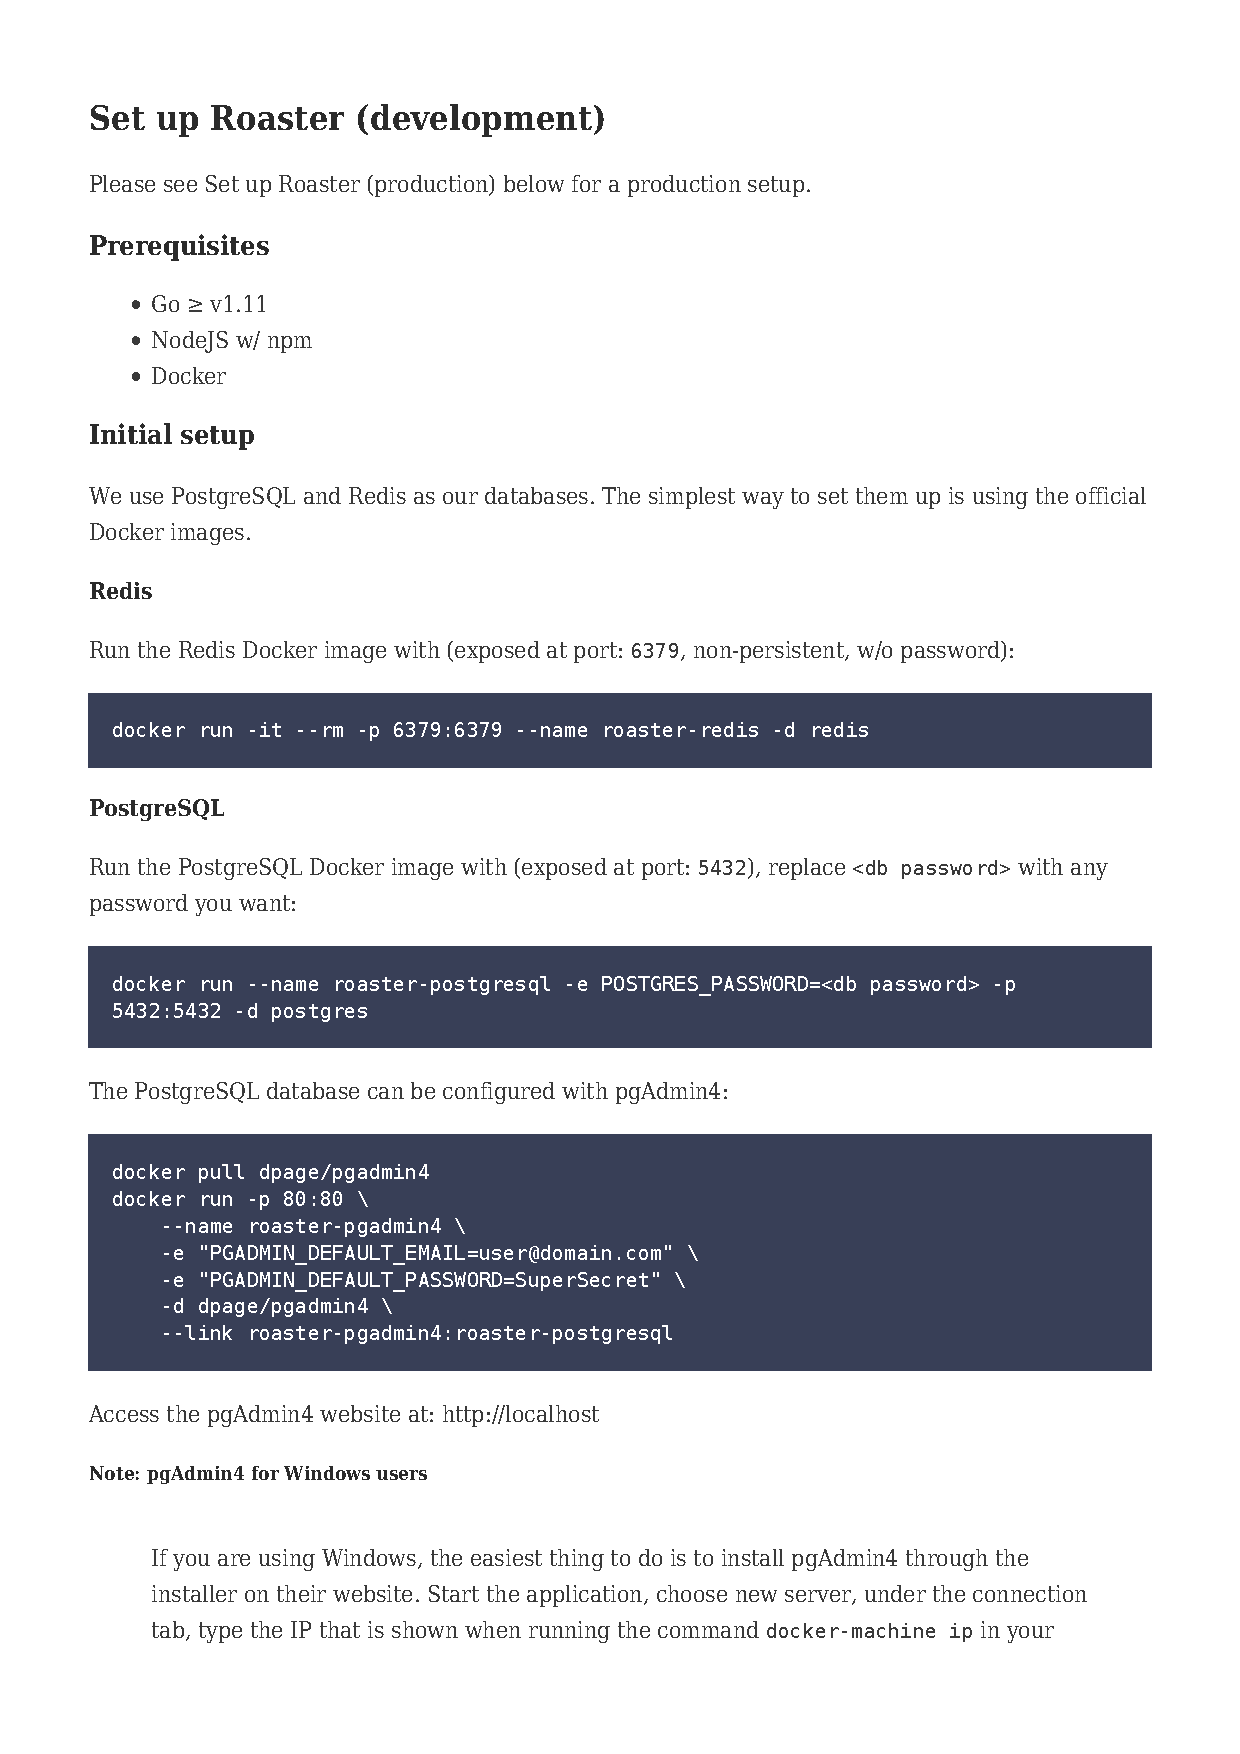
\includepdf[page=-]{install.pdf}
\end{appendix}

% Here follows some good to have examples.
\if false

\begin{figure}[H]
    \centering
    \includegraphics[width=6cm]{xxx.png}
    \caption{Lalalala.}
    \label{fig:my_label}
\end{figure}

\begin{verbatim}
PaymentTest > entitledFullAmount[ID: 505] FAILED
    java.lang.AssertionError: expected:<4960> but was:<5960>
        at org.junit.Assert.fail(Assert.java:88)
        at org.junit.Assert.failNotEquals(Assert.java:834)
        at org.junit.Assert.assertEquals(Assert.java:645)
        at org.junit.Assert.assertEquals(Assert.java:631)
        at PaymentTest.entitledFullAmount(PaymentTest.java:164)
\end{verbatim}

\begin{table}[H]
\centering
\caption{API endpoints and their methods}
\begin{tabular}{|clcl|}
\hline
\textbf{Method}              & \textbf{Endpoint}                             & \textbf{Access}              & \textbf{Description}                 \\ \hline
\multicolumn{1}{|c|}{GET}    & \multicolumn{1}{l|}{/}                        & \multicolumn{1}{c|}{N/A}     & Home page                            \\
\multicolumn{1}{|c|}{GET}    & \multicolumn{1}{l|}{/login}                   & \multicolumn{1}{c|}{N/A}     & View customer login page                      \\
\multicolumn{1}{|c|}{POST}   & \multicolumn{1}{l|}{/login}                   & \multicolumn{1}{c|}{N/A}     & Login customer user                           \\
\multicolumn{1}{|c|}{GET}    & \multicolumn{1}{l|}{/register}                & \multicolumn{1}{c|}{N/A}     & View customer register page                   \\
\multicolumn{1}{|c|}{POST}   & \multicolumn{1}{l|}{/register}                & \multicolumn{1}{c|}{N/A}     & Register customer user                        \\
\multicolumn{1}{|c|}{GET}    & \multicolumn{1}{l|}{/user}                    & \multicolumn{1}{c|}{C, W, A} & View user page                       \\
\multicolumn{1}{|c|}{POST}   & \multicolumn{1}{l|}{/user}                    & \multicolumn{1}{c|}{C, W, A} & Set user information                 \\
\multicolumn{1}{|c|}{GET}    & \multicolumn{1}{l|}{/article?id=\{0..n\}}     & \multicolumn{1}{c|}{C, W, A} & Get specific article by ID           \\
\multicolumn{1}{|c|}{POST}   & \multicolumn{1}{l|}{/cart}                    & \multicolumn{1}{c|}{C}       & Add artice to cart                   \\
\multicolumn{1}{|l|}{DELETE} & \multicolumn{1}{l|}{/cart?pos=\{0..n\}}       & \multicolumn{1}{c|}{C}       & Delete article from cart by position \\
\multicolumn{1}{|l|}{DELETE} & \multicolumn{1}{l|}{/cart}                    & \multicolumn{1}{c|}{C}       & Delete whole cart                    \\
\multicolumn{1}{|c|}{GET}    & \multicolumn{1}{l|}{/cart}                    & \multicolumn{1}{c|}{C}       & View cart                            \\
\multicolumn{1}{|c|}{PUT}    & \multicolumn{1}{l|}{/cart}                    & \multicolumn{1}{c|}{C}       & Order items in cart                  \\
\multicolumn{1}{|c|}{GET}    & \multicolumn{1}{l|}{/order}                   & \multicolumn{1}{c|}{W, A}    & View current orders                  \\
\multicolumn{1}{|c|}{GET}    & \multicolumn{1}{l|}{/order?id=\{0..n\}}       & \multicolumn{1}{c|}{W, A}    & View order by ID                     \\
\multicolumn{1}{|c|}{GET}    & \multicolumn{1}{l|}{/warehouse}               & \multicolumn{1}{c|}{W}       & Warehouse user home page             \\
\multicolumn{1}{|c|}{GET}    & \multicolumn{1}{l|}{/admin}                   & \multicolumn{1}{c|}{A}       & Admin user home page                 \\
\multicolumn{1}{|c|}{PUT}    & \multicolumn{1}{l|}{/order?id=\{0..n\}}       & \multicolumn{1}{c|}{W}       & Accept order by ID                   \\
\multicolumn{1}{|c|}{GET}    & \multicolumn{1}{l|}{/user?id=\{0..n\}}        & \multicolumn{1}{c|}{A}       & Display user by ID                   \\
\multicolumn{1}{|c|}{GET}    & \multicolumn{1}{l|}{/search?query=\{string\}}        & \multicolumn{1}{c|}{N/A}       & Search for article                   \\
\multicolumn{1}{|c|}{POST}   & \multicolumn{1}{l|}{/register?type=admin}     & \multicolumn{1}{c|}{A}       & Register new admin user              \\
\multicolumn{1}{|c|}{POST}   & \multicolumn{1}{l|}{/register?type=warehouse} & \multicolumn{1}{c|}{A}       & Register new warehouse user          \\
\multicolumn{1}{|c|}{POST}   & \multicolumn{1}{l|}{/register?type=customer}  & \multicolumn{1}{c|}{A}       & Register new customer user           \\ \hline
\end{tabular}
\end{table}
\fi
\end{document}
